%% LyX 2.2.3 created this file.  For more info, see http://www.lyx.org/.
%% Do not edit unless you really know what you are doing.
%\documentclass[english]{article}

\documentclass[final,12pt]{colt2018} % Anonymized submission
% \documentclass{colt2017} % Include author names

% The following packages will be automatically loaded:
% amsmath, amssymb, natbib, graphicx, url, algorithm2e

\title[Optimization with Oracles]{Efficient Convex Optimization with Membership Oracles}
\usepackage{times}
 % Use \Name{Author Name} to specify the name.
 % If the surname contains spaces, enclose the surname
 % in braces, e.g. \Name{John {Smith Jones}} similarly
 % if the name has a "von" part, e.g \Name{Jane {de Winter}}.
 % If the first letter in the forenames is a diacritic
 % enclose the diacritic in braces, e.g. \Name{{\'E}louise Smith}

 % Two authors with the same address
  % \coltauthor{\Name{Author Name1} \Email{abc@sample.com}\and
  %  \Name{Author Name2} \Email{xyz@sample.com}\\
  %  \addr Address}

 % Three or more authors with the same address:
 % \coltauthor{\Name{Author Name1} \Email{an1@sample.com}\\
 %  \Name{Author Name2} \Email{an2@sample.com}\\
 %  \Name{Author Name3} \Email{an3@sample.com}\\
 %  \addr Address}


%\usepackage[latin9]{inputenc}
%\usepackage{geometry}
%\geometry{verbose,lmargin=3cm,rmargin=3cm}
\usepackage{tipa}
\usepackage{tipx}
\usepackage{amsmath}
%\usepackage{amsthm}

%\makeatletter
%%%%%%%%%%%%%%%%%%%%%%%%%%%%%% Textclass specific LaTeX commands.
%\numberwithin{equation}{section}
%\numberwithin{figure}{section}
%\theoremstyle{plain}
%\newtheorem{thm}{\protect\theoremname}
%  \theoremstyle{definition}
%  \newtheorem{defn}[thm]{\protect\definitionname}
%  \theoremstyle{plain}
%  \newtheorem{lem}[thm]{\protect\lemmaname}

%%%%%%%%%%%%%%%%%%%%%%%%%%%%%% User specified LaTeX commands.
%%%%%%%%%%%%%%%%%%Commenting macros%%%%%%%%%%%%%%%%%
\def\final{0}  % set this to 1 to get a comment-free version

\ifnum\final=0  %namely if we allow comments in the output
\newcommand{\note}[1]{[{\tiny \bf #1}]\marginpar{*}}
\newcommand{\sidecomment}[1]{\marginpar{\tiny #1}}
\else % in this case [final=1] we don't want any comments to show
\newcommand{\note}[1]{}
\newcommand{\sidecomment}[1]{}
\fi  %ok, we're done with defining comment macros
%%%%%%%%%%%%%%%%%%%%%%%%%%%%%%%%%%%%%%%%%%%%%%%%%%%%

%\usepackage[lined,boxed,ruled,norelsize,algo2e]{algorithm2e}

\usepackage{amsfonts}
\usepackage{tikz}
\usetikzlibrary{shapes,arrows,arrows.meta}

\makeatletter
\newcommand{\xleftrightarrow}[2][]{\ext@arrow 3359\leftrightarrowfill@{#1}{#2}}
\newcommand{\xdashrightarrow}[2][]{\ext@arrow 0359\rightarrowfill@@{#1}{#2}}
\newcommand{\xdashleftarrow}[2][]{\ext@arrow 3095\leftarrowfill@@{#1}{#2}}
\newcommand{\xdashleftrightarrow}[2][]{\ext@arrow 3359\leftrightarrowfill@@{#1}{#2}}
\def\rightarrowfill@@{\arrowfill@@\relax\relbar\rightarrow}
\def\leftarrowfill@@{\arrowfill@@\leftarrow\relbar\relax}
\def\leftrightarrowfill@@{\arrowfill@@\leftarrow\relbar\rightarrow}
\def\arrowfill@@#1#2#3#4{%
  $\m@th\thickmuskip0mu\medmuskip\thickmuskip\thinmuskip\thickmuskip
   \relax#4#1
   \xleaders\hbox{$#4#2$}\hfill
   #3$%
}

% alternative to arrow
\pgfarrowsdeclare{tonew}{tonew}
{
  \ifdim\pgfgetarrowoptions{tonew}=-1pt%
    \pgfutil@tempdima=0.84pt%
    \advance\pgfutil@tempdima by1.3\pgflinewidth%
    \pgfutil@tempdimb=0.21pt%
    \advance\pgfutil@tempdimb by.625\pgflinewidth%
  \else%
    \pgfutil@tempdima=\pgfgetarrowoptions{tonew}%
    \pgfarrowsleftextend{+-0.8\pgfutil@tempdima}%
    \pgfarrowsrightextend{+0.2\pgfutil@tempdima}%
  \fi%
}
{
  \ifdim\pgfgetarrowoptions{tonew}=-1pt%
    \pgfutil@tempdima=0.28pt%
    \advance\pgfutil@tempdima by.3\pgflinewidth%
    \pgfutil@tempdimb=0pt,%
  \else%
    \pgfutil@tempdima=\pgfgetarrowoptions{tonew}%
    \multiply\pgfutil@tempdima by 100%
    \divide\pgfutil@tempdima by 375%
    \pgfutil@tempdimb=0.4\pgflinewidth%
  \fi%
  \pgfsetdash{}{+0pt}
  \pgfsetroundcap
  \pgfsetroundjoin
  \pgfpathmoveto{\pgfpointorigin}
  \pgflineto{\pgfpointadd{\pgfpoint{0.75\pgfutil@tempdima}{0bp}}
                         {\pgfqpoint{-2\pgfutil@tempdimb}{0bp}}}
  \pgfusepathqstroke
  \pgfsetlinewidth{0.8\pgflinewidth}
  \pgfpathmoveto{\pgfpointadd{\pgfqpoint{-3\pgfutil@tempdima}{4\pgfutil@tempdima}}
                             {\pgfqpoint{\pgfutil@tempdimb}{0bp}}}
  \pgfpathcurveto
  {\pgfpointadd{\pgfqpoint{-2.75\pgfutil@tempdima}{2.5\pgfutil@tempdima}}
               {\pgfqpoint{0.5\pgfutil@tempdimb}{0bp}}}
  {\pgfpointadd{\pgfqpoint{0pt}{0.25\pgfutil@tempdima}}
               {\pgfqpoint{-0.5\pgfutil@tempdimb}{0bp}}}
  {\pgfpointadd{\pgfqpoint{0.75\pgfutil@tempdima}{0pt}}
               {\pgfqpoint{-\pgfutil@tempdimb}{0bp}}}
  \pgfpathcurveto
  {\pgfpointadd{\pgfqpoint{0pt}{-0.25\pgfutil@tempdima}}
               {\pgfqpoint{-0.5\pgfutil@tempdimb}{0bp}}}
  {\pgfpointadd{\pgfqpoint{-2.75\pgfutil@tempdima}{-2.5\pgfutil@tempdima}}
               {\pgfqpoint{0.5\pgfutil@tempdimb}{0bp}}}
  {\pgfpointadd{\pgfqpoint{-3\pgfutil@tempdima}{-4\pgfutil@tempdima}}
               {\pgfqpoint{\pgfutil@tempdimb}{0bp}}}
  \pgfusepathqstroke
}

% alias alternative to arrow
\pgfarrowsdeclarealias{<new}{>new}{tonew}{tonew}
\pgfsetarrowoptions{tonew}{-1pt}
\pgfkeys{/tikz/.cd, arrowhead/.default=-1pt, arrowhead/.code={
  \pgfsetarrowoptions{tonew}{#1},
}}
\makeatother

\makeatother

%\usepackage{babel}
  \providecommand{\definitionname}{Definition}
  \providecommand{\lemmaname}{Lemma}
\providecommand{\theoremname}{Theorem}

%\makeatletter
%%%%%%%%%%%%%%%%%%%%%%%%%%%%%% Textclass specific LaTeX commands.
%\numberwithin{equation}{section}
%\numberwithin{figure}{section}
%\theoremstyle{plain}
\newtheorem{thm}{\protect\theoremname}
%  \theoremstyle{definition}
\newtheorem{defn}[thm]{\protect\definitionname}
%  \theoremstyle{plain}
\newtheorem{lem}[thm]{\protect\lemmaname}

 % Authors with different addresses:
 \coltauthor{\Name{Yin Tat Lee} \Email{yintat@uw.edu}\\
 \addr University of Washington
 \AND
 \Name{Aaron Sidford} \Email{sidford@stanford.edu}\\
 \addr Stanford University
\AND
\Name{Santosh S. Vempala} \Email{vempala@gatech.edu}\\
\addr Georgia Tech
 }

\begin{document}

\maketitle

\begin{abstract}
We consider the problem of minimizing a convex function over a convex
set given access only to an evaluation oracle for the function and
a membership oracle for the set. We give a simple algorithm which
solves this problem with $\tilde{O}(n^{2})$ oracle calls and $\tilde{O}(n^{3})$
additional arithmetic operations. Using this result, we obtain more
efficient reductions among the five basic oracles for convex sets
and functions defined by 
\citet{GLS}.\footnote{Extended abstract. Full version appears as [arXiv:1706.07357]}

% Copy paste version
%We consider the problem of minimizing a convex function over a convex
%set given access only to an evaluation oracle for the function and
%a membership oracle for the set. We give a simple algorithm which
%solves this problem with $\tilde{O}(n^{2})$ oracle calls and $\tilde{O}(n^{3})$
%additional arithmetic operations. Using this result, we obtain more
%efficient reductions among the five basic oracles for convex sets
%and functions defined by Gr{\"o}tschel, Lov{\'a}sz, and Schrijver (1988).
\end{abstract}

\begin{keywords}
Optimization, Membership, Separation, Violation, Validity, Subgradient
\end{keywords}


%\begin{document}
\global\long\def\defeq{\stackrel{\mathrm{{\scriptscriptstyle def}}}{=}}
\global\long\def\norm#1{\left\Vert #1\right\Vert }
\global\long\def\R{\mathbb{R}}
 \global\long\def\Rn{\mathbb{R}^{n}}
\global\long\def\tr{\mathrm{Tr}}
\global\long\def\diag{\mathrm{diag}}
\global\long\def\vol{\mathrm{Vol}}
\global\long\def\E{\mathbb{E}}
\global\long\def\time{\mathcal{T}}
\global\long\def\SO{\text{SO}}
\global\long\def\linspan{\mbox{span}}
\global\long\def\eps{\varepsilon}
\global\long\def\ortho{\perp}
\global\long\def\giventhat{\mid}
\global\long\def\RR{\mathbb{R}}
\global\long\def\card#1{\lvert#1\rvert}
\global\long\def\oproj{\mbox{proj}}
\global\long\def\proj{\pi}
\global\long\def\poly{\mbox{poly}}
\global\long\def\suchthat{\mathrel{:}}
\global\long\def\abs#1{\left|#1\right|}
\global\long\def\ZZ{\mathbb{Z}}
\global\long\def\width{\mbox{width}}
\global\long\def\otilde{\widetilde{O}}
\global\long\def\indicfunc#1{1_{#1}}




%\author{Yin Tat Lee\thanks{Microsoft Research, yile@microsoft.com} \and Aaron Sidford\thanks{Stanford University, sidford@stanford.edu} \and Santosh S. Vempala \thanks{Georgia Tech, vempala@gatech.edu}}
%\maketitle
%\begin{abstract}
%We consider the problem of minimizing a convex function over a convex
%set given access only to an evaluation oracle for the function and
%a membership oracle for the set. We give a simple algorithm which
%solves this problem with $\otilde(n^{2})$ oracle calls and $\otilde(n^{3})$
%additional arithmetic operations. Using this result, we obtain more
%efficient reductions among the five basic oracles for convex sets
%and functions defined by Gr�tschel, Lov\textipa{a}sz and Schrijver
%\cite{GLS}.
%\end{abstract}
%\thispagestyle{empty}\newpage
%\clearpage \setcounter{page}{1}

% !TeX root = main.tex
\section{Introduction}
\label{sec:intro}
Generative models are often trained in an unsupervised fashion, fitting a model $q$ to a set of observed data $x_P \subseteq X$ drawn iid from some true distribution $p$ on $x\in X$. Now, of course $p$ may not exactly belong to family $Q$ of probability distributions being fit, whether $Q$ consists of Gaussians mixture models, Markov models, or even neural networks of bounded size. We first discuss the limitations of generative modeling without feedback, and then discuss our model and results.

%\subsection{Limitations of Generative Modeling from Positive Examples Alone}
Consider fitting a generative model on a text corpus consisting partly of poetry written by four-year-olds and partly of mathematical publications from the {\em Annals of Mathematics}. Suppose that learning to generate a poem that looks like it was written by a child was easier than learning to generate a novel mathematical article with a correct, nontrivial statement. If the generative model pays a high price for generating unrealistic examples, then it may be better off learning to generate children's poetry than mathematical publications. However, without negative feedback, it may be difficult for a neural network or any other model to know that the mathematical articles it is generating are stylistically similar to the mathematical publications but do not contain valid proofs.\footnote{This is excluding clearly fake articles published without proper review in lower-tier venues \citep{LabbeL13}.} 

As a simpler example, the classic Markovian ``trigram model'' of natural language assigns each word a fixed probability conditioned only on the previous two words. Prior to recent advances in deep learning, for decades the trigram model and its variant were the workhorses of language modeling, assigning much greater likelihood to natural language corpora than numerous linguistically motivated grammars and other attempts \citep{Rosenfeld00}. However, text sampled from a trigram is typically nonsensical, e.g., the following text was randomly generated from a trigram model fit on a corpus of text from the Wall Street Journal \citep{JurafskyM09}:
\begin{quote}
They also point to ninety nine point six billion dollars from two hundred
four oh six three percent of the rates of interest stores as Mexico and
gram Brazil on market conditions. 
\end{quote}

In some applications, like text compression using a language model \citep{WittenNC87}, maximizing likelihood is equivalent to optimizing compression. However, in many  applications involving generation, such nonsense is costly and unacceptable. Now, of course it is possible to always generate valid data by returning random training examples, but this is simply overfitting and not learning. Alternatively, one could incorporate human-in-the-loop feedback such as through crowdsourcing, into the generative model to determine what is a valid, plausible sentence.

In some domains, validity could be determined automatically. Consider a Markovian model of a well-defined concept such as mathematical formulas that compile in \LaTeX{}. Now, consider a $n$-gram Markovian character model which the probability of each subsequent character is determined by the previous $n$ characters. For instance, the expression \$\{2+\{x-y\}\$ is invalid in \LaTeX{} due to mismatched braces. For this problem, a \LaTeX{} compiler may serve as a validity oracle. Various $n$-gram models can be fit which only generate valid formulas. To address mismatched braces, for example, one such model would ensure that it always closed braces within $n$ characters of opening, and had no nested braces. While an $n$-gram model will not perfectly model the true distribution over valid \LaTeX{} formulas, for certain generative purposes one may prefer an $n$-gram model that generates valid formulas over one that assigns greater likelihood to the training data but generates invalid formulas. 

Figure \ref{fig:rectangle} illustrates a simple case of learning a rectangle model for data which is not uniform over a rectangle. A maximum likelihood model would necessarily be the smallest rectangle containing all the data, but most examples generated from this distribution may be invalid. Instead a smaller rectangle, as illustrated in the figure, may be desired.

\begin{figure}[h]\label{fig:rectangle}
\centering
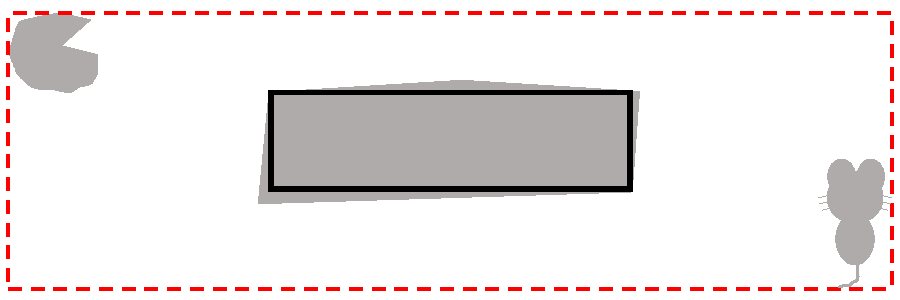
\includegraphics[width=3in]{fig.pdf}
\caption{Example where the underlying distribution $p$ is uniform over the (gray) valid regions. The solid rectangle maximizes our objective since it does not output nonsense (is supported only within the grey matter) and is closest to the $p$ (covers the maximum amount of grey matter). In contrast, the standard maximum likelihood (dashed red) rectangle must fully contain the observed samples, thus generating invalid points most of the time.  }
\end{figure}

Motivated by these observations, we evaluate a generative model $q$ on two axes. First is {\em coverage}, which is related to the probability assigned to future examples drawn from the true distribution $p$. Second is {\em validity}, defined as the probability that random examples generated from $q$ meet some validity requirement. Formally, we measure coverage in terms of a bounded {\em loss}:
$$\Loss(p,q)=\E_{x \sim p}[L(q_x)],$$
where $L:[0,1]\rightarrow [0,M]$ is a bounded decreasing function such as the capped log-loss $L(q_x)=\min(M, \log 1/q_x)$. % or $L(q_x)=\log 1/(q_x+\exp(-M))$. 
A bounded loss has the advantages of being efficiently estimable, and also it enables a model to assign 0 probability to one example (e.g., an outlier or error) if it greatly increases the likelihood of all other data. Validity is defined with respect to a set $V \subseteq X$, and $q(V)$ is the probability that a random example generated from $q$ lies within $V$. 

Clearly, there is a tradeoff between coverage and validity. We first focus on the case of (near) perfect validity. A Valid Generative Modeling (VGM) algorithm if it outputs, for a family of distributions $Q$ over $X$, if it outputs $\hat{q}$ with (nearly) perfect validity and whose loss is nearly as good as the loss of the best valid $q\in Q$. More precisely, $A$ is a VGM learner of $Q$ if for any nonempty valid subset $V \subseteq X$, any probability distribution $p$ over $V$, and any $\eps>0$, $A$ uses $n$ random samples from $p$ and makes $m$ membership oracle calls to $V$ and outputs a distribution $\hat{q}$ such that, $$\Loss(p, \hat{q}) \leq \min_{q \in Q: q(V)=1}\Loss(p,q) + \eps ~\text{ and }~\hat{q}(V)\geq 1-\eps.$$ 
We aim for our learner to be sample and query efficient, requiring that $n$ and $m$ are polynomial in $M, 1/\eps$ and a measure of complexity of our distribution class $Q$.
Furthermore, we would like our algorithms to be computationally efficient, with a runtime polynomial in the size of the data, namely the $n + m$ training examples. 
A more formal description of the problem is available in Section~\ref{sec:problem}.

$A$ is said to be {\em proper} if it always outputs $\hat{q}\in Q$ and {\em improper} otherwise.
In Section~\ref{sec:impossibility}, we first show that efficient proper learning for VGM is impossible. This is an information-theoretic result, meaning that even given infinite runtime and positive samples, one still cannot solve the VGM problem. Interestingly, this is different from binary classification, where it is possible to statistically learn from iid examples without a membership oracle.

Our first main positive result is an efficient (improper) learner for VGM. The algorithm relies on a subroutine that solves the following {\em Generative Modeling with Negatives} (GMN) problem: given sets $X_P, X_N \subset X$ of positive and negative examples, find the probability distribution $q \in Q$ which minimizes $\sum_{x \in X_P} L(q(x))$ subject to the constraint that $q(X_N)=0$. For simplicity, we present our algorithm for the case that the distribution family $Q$ is finite, giving sample and query complexity bounds that are logarithmic in terms of $|Q|$. However, as we show in Section~\ref{sec:infinite-families}, all of our results extend to infinite families $Q$. It follows that if one has a computationally efficient algorithm for the GMN problem for a distribution family $Q$, then our reduction gives a computationally efficient VGM learning algorithm for $Q$.

Our second positive result is an algorithm that minimizes $\Loss(p,q)$ subject to a relaxed validity constraint comparing against the optimal distribution that has validity $q(V)$ at least $1-\alpha$ for some $\alpha>0$. We show in Section~\ref{sec:partial-validity} that even in this more general setting, it is possible to obtain an algorithm that is statistically efficient but may not be computationally efficient. An important open question is whether there exists a computationally efficient algorithm for this problem when given access to an optimization oracle, as was the case for our algorithm for VGM.

\subsection{Related Work}
\cite{KearnsMRRSS94} showed how to learn distributions from positive examples in the realizable setting, i.e., where the true distribution is assumed to belong to the class being learned. In the same sense as their work is similar to PAC learning \citet{Valiant84} of distributions, our work is like agnostic learning \citet{KearnsSS94} in which no assumption on the true distribution is made. 

Generative Adversarial Networks (GANs)~\cite{GoodfellowPMXWOCB14} are an approach for generative modeling from positive examples alone, in which a generative model is trained against a discriminator that aims to distinguish real data from generated data. In some domains, GANs have been shown to outperform other methods at generating realistic-looking examples. Several shortcomings of GANs have been observed \citet{AroraRZ18}, and GANs are still subject to the theoretical limitations we argue are inherent to any model trained without a validity oracle. 

In supervised learning, there is a rich history of learning theory with various types of queries, including membership which are not unlike our (in)validity oracle. Under various assumptions, queries have been shown to facilitate the learning of complex classes such as finite automata \citet{Angluin88} and DNFs \citet{Jackson97}. See the survey of \cite{Angluin92} for further details.  Interestingly, \cite{Feldman09} has shown that for agnostic learning, i.e., without making assumptions on the generating distribution, the addition of membership queries does not enhance what is learnable beyond random examples alone. 
Supervised learning also has a large literature around active learning, showing how the ability to query examples reduces the sample complexity of many algorithms. See the survey of \cite{Hanneke14}. Note that the aim here is typically to save examples and not to expand what is learnable.
 
More sophisticated models, e.g., involving neural networks, can mitigate the invalidity problem as they often generate more realistic natural language and have even been demonstrated to generate \LaTeX{} that nearly compiles \citep{Karpathy15} or nearly valid Wikipedia markdown. However, longer strings generated are unlikely to be valid. For example, \cite{Karpathy15} shows generated markdown which includes:
\begin{quote}
==Access to ''rap===
The current history of the BGA has been [[Vatican Oriolean Diet]], British Armenian, published in 1893.  While actualistic such conditions such as the [[Style Mark Romanians]] are still nearly not the loss.
\end{quote}

Even ignoring the mismatched quotes and equal signs, note that this example has two so-called ``red links'' to two pages that do not exist. Without checking, it was not obvious to us whether or not Wikipedia had pages titled {\em Vatican Oriolean Diet} or {\em Style Mark Romanians}. In some applications, one may or may not want to disallow red links. In the case that they are considered valid, one may seek a full generative model of what might plausibly occur inside of brackets, as the neural network has learned in this case. If they are disallowed, a model might memorize links it has seen but not generate new ones. A validity oracle can help the learner identify what it should avoid generating.

 In practice, \cite{KusnerPH17} discuss how generative models from neural networks (in particular autoencoders) often generate invalid sequences. 
\cite{JanzWPKH18} learn the validity of examples output by a generative model using oracle feedback. 


\acks{The authors thank Sebastien Bubeck, Ben Cousins, Sham M. Kakade and
Ravi Kannan for helpful discussions, and Yan Kit Chim for making the
illustrations. Finally, we thank Xiaodi Wu for pointing out some typos
in a previous version of the paper.}

%\bibliographystyle{plain}
\bibliography{lee18}

\end{document}
